\begin{frame}\addtocounter{framenumber}{-1}
\frametitle{The CMS detector}
\begin{center}
\vphantom{Iron return yoke (red) interspersed with muon chambers (gray)}~\\
\vphantom{detects charged particles going through (only muons as other particles are stopped by ECAL or HCAL)}~

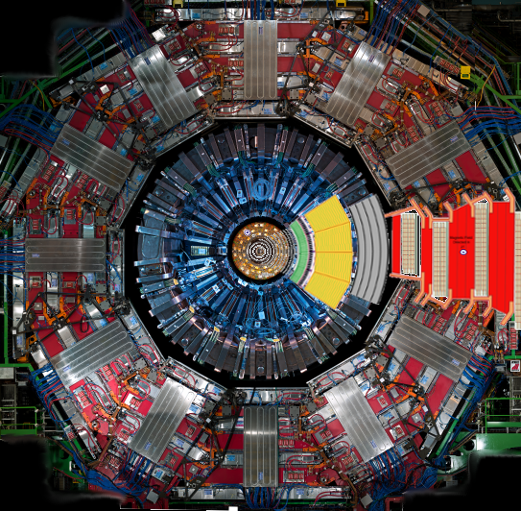
\includegraphics[width=\textwidth,height=\graphh,keepaspectratio]{/home/torterotot/Documents/PhD-Thesis/tex/slides/LHC-CMS/CMS/slice_on_photo.png}

$\longleftarrow \SI{15}{\meter} \longrightarrow$
\end{center}
\end{frame}
